\documentclass[11pt,a4paper]{article}

\usepackage[a4paper,margin=23mm]{geometry}
\usepackage[T1]{fontenc}
\usepackage[utf8]{inputenc}
\usepackage{lmodern}
\usepackage{microtype}
\usepackage{amsmath,amssymb,mathtools,bm}
\usepackage{graphicx}
\usepackage{booktabs}
\usepackage{array}
\usepackage{enumitem}
\usepackage{xcolor}
\usepackage{hyperref}
\usepackage{caption}
\usepackage{subcaption}
\usepackage{siunitx}

\hypersetup{
  colorlinks=true,
  linkcolor=blue!55!black,
  citecolor=blue!55!black,
  urlcolor=blue!55!black
}

\setlength{\parindent}{0pt}
\setlength{\parskip}{0.55em}
\setlist[itemize]{topsep=0.25em,itemsep=0.15em}
\setlist[enumerate]{topsep=0.25em,itemsep=0.15em}

\newcommand{\id}{i_d}
\newcommand{\iq}{i_q}
\newcommand{\ie}{i_{\mathrm{exc}}}
\newcommand{\Rs}{R_s}
\newcommand{\Rexc}{R_{\mathrm{exc}}}
\newcommand{\Ld}{L_d}
\newcommand{\Lq}{L_q}
\newcommand{\Lexc}{L_{\mathrm{exc}}}
\newcommand{\psipm}{\psi_{\mathrm{pm}}}
\newcommand{\w}{\omega}
\newcommand{\Imax}{I_{\max}}
\newcommand{\Umax}{U_{\max}}
\newcommand{\Pmax}{P_{\mathrm{Cu,max}}}
\newcommand{\T}{\mathsf{T}}
\newcommand{\R}{\mathbb{R}}
\newcommand{\vct}[1]{\bm{#1}}
\newcommand{\mat}[1]{\bm{#1}}

\title{\textbf{Geometry of Voltage Limits and Optimal Current Allocation in PMSM and EESM Drives}\\[0.4em]
\large From quadratic forms, eigenvectors and conic sections to MTPA, field weakening and MTPV}
\author{Conceptual technical note}
\date{September 2026}

\begin{document}

\maketitle

\begin{abstract}
This note develops a geometric interpretation of steady-state operating limits for permanent-magnet synchronous machines (PMSM/IPMSM) and electrically excited synchronous machines (EESM). The goal is not merely to state the familiar current circles, voltage ellipses, torque hyperbolas and MTPA/MTPV conditions, but to derive them from first principles and explain why their geometry has exactly the observed shape. The central mathematical object is the quadratic form. Its eigenvalues, eigenvectors, determinant, rank and singular-value decomposition are connected directly to the center, orientation, principal axes and degeneracies of the corresponding current-space surfaces. For the PMSM, the stator-voltage limit is shown to be an ellipse in the $(i_d,i_q)$ plane. For the EESM, adding excitation current as a third degree of freedom turns the family of voltage ellipses into an oblique elliptic cylinder in $(i_d,i_q,i_{\mathrm{exc}})$ space, while a copper-loss constraint becomes a true ellipsoid. MTPA and MTPV are interpreted as tangency conditions between level sets and constraints. A key EESM result is that a pure stator-voltage-only MTPV problem is generally not bounded in the simplified linear model because the voltage quadratic form has a null-space direction; a finite optimum requires an additional loss, current, excitation or thermal constraint. Numerical implications for Delaunay-based iso-level searches and three-dimensional isosurface visualization are discussed at the end.
\end{abstract}

\tableofcontents
\newpage

\section{What this paper is trying to make intuitive}

A typical current-space diagram of a synchronous machine contains several curves that are often memorized as separate facts:

\begin{itemize}
  \item a current circle,
  \item a voltage ellipse,
  \item torque hyperbolas,
  \item an MTPA trajectory,
  \item a field-weakening trajectory,
  \item and an MTPV trajectory.
\end{itemize}

The deeper point is that these are not unrelated constructions. They arise from only a few recurring ideas:

\begin{enumerate}
  \item \textbf{A norm constraint} such as $\|\vct u\|=\Umax$ is a circle in voltage space.
  \item \textbf{A linear or affine map} from current space to voltage space pulls that circle back into an ellipse or, in higher dimensions, into a cylindrical quadratic surface.
  \item \textbf{A quadratic form} $\vct x^\T \mat Q\vct x$ describes direction-dependent ``distance''. Eigenvectors identify directions in which this distorted distance decouples; eigenvalues tell how expensive motion is in those directions.
  \item \textbf{Constrained optima occur at tangencies.} If one level set is pushed outward until it just touches a constraint, their normal vectors are parallel. This is the geometric meaning of Lagrange multipliers and, with inequalities, the Karush--Kuhn--Tucker (KKT) conditions.
\end{enumerate}

The same mathematical machinery will be used first in two dimensions for the PMSM and then in three dimensions for the EESM.

\paragraph{Guiding analogy: a distorted ruler.}
The ordinary Euclidean expression $x_1^2+x_2^2$ measures squared distance with a ruler that treats every direction equally. A quadratic form $\vct x^\T\mat Q\vct x$ is a ruler that may stretch, compress and rotate the coordinate system. A ``circle'' measured with that ruler appears as an ellipse in the original coordinates. Eigenvectors are the ruler's natural directions; eigenvalues tell how strongly each direction is weighted.

\section{Mathematical toolkit: quadratic forms before machines}

\subsection{From circles to ellipses}

Consider the set
\begin{equation}
  \vct x^\T \mat Q\vct x = c,
  \qquad c>0,
  \label{eq:quadform-level}
\end{equation}
where $\mat Q\in\R^{2\times2}$ is real and symmetric,
\begin{equation}
  \mat Q =
  \begin{bmatrix}
    a & b\\
    b & c_q
  \end{bmatrix}.
\end{equation}
The subscript on $c_q$ avoids confusion with the level value $c$.

If $\mat Q=\mat I$, then \eqref{eq:quadform-level} is the circle $x_1^2+x_2^2=c$. If $\mat Q$ is diagonal but not proportional to the identity,
\begin{equation}
  \lambda_1 x_1^2 + \lambda_2 x_2^2 = c,
\end{equation}
then dividing by $c$ gives
\begin{equation}
  \frac{x_1^2}{c/\lambda_1} + \frac{x_2^2}{c/\lambda_2}=1.
\end{equation}
Hence the semi-axis lengths are
\begin{equation}
  a_1=\sqrt{\frac{c}{\lambda_1}},
  \qquad
  a_2=\sqrt{\frac{c}{\lambda_2}}.
  \label{eq:axis-length-basic}
\end{equation}
The larger the coefficient $\lambda_i$, the shorter the corresponding axis. This makes intuitive sense: if the quadratic form penalizes motion in one direction strongly, one can move only a small geometric distance before reaching the same level $c$.

\subsection{Why eigenvectors are the ellipse axes}

Because $\mat Q$ is real and symmetric, the spectral theorem guarantees an orthonormal eigenbasis:
\begin{equation}
  \mat Q = \mat V\mat\Lambda\mat V^\T,
  \qquad
  \mat\Lambda=\operatorname{diag}(\lambda_1,\lambda_2),
\end{equation}
where the columns $\vct v_1,\vct v_2$ of $\mat V$ are orthonormal eigenvectors.

Introduce rotated coordinates
\begin{equation}
  \vct z = \mat V^\T\vct x.
\end{equation}
Then
\begin{align}
  \vct x^\T\mat Q\vct x
  &= \vct x^\T\mat V\mat\Lambda\mat V^\T\vct x\\
  &= \vct z^\T\mat\Lambda\vct z\\
  &= \lambda_1 z_1^2+\lambda_2 z_2^2.
\end{align}
There is no mixed term $z_1z_2$. The eigenbasis is therefore exactly the coordinate system in which the quadratic form decouples into two independent squared coordinates. That is why the eigenvectors are the principal axes.

A still simpler way to see the same fact is to move only along one eigenvector, $\vct x=t\vct v_i$. Then
\begin{equation}
  \vct x^\T\mat Q\vct x
  = t^2\vct v_i^\T\mat Q\vct v_i
  = t^2\lambda_i.
\end{equation}
Reaching the level $c$ requires
\begin{equation}
  |t|=\sqrt{\frac{c}{\lambda_i}},
\end{equation}
which is exactly the semi-axis length in that eigenvector direction.

\begin{figure}[htbp]
  \centering
  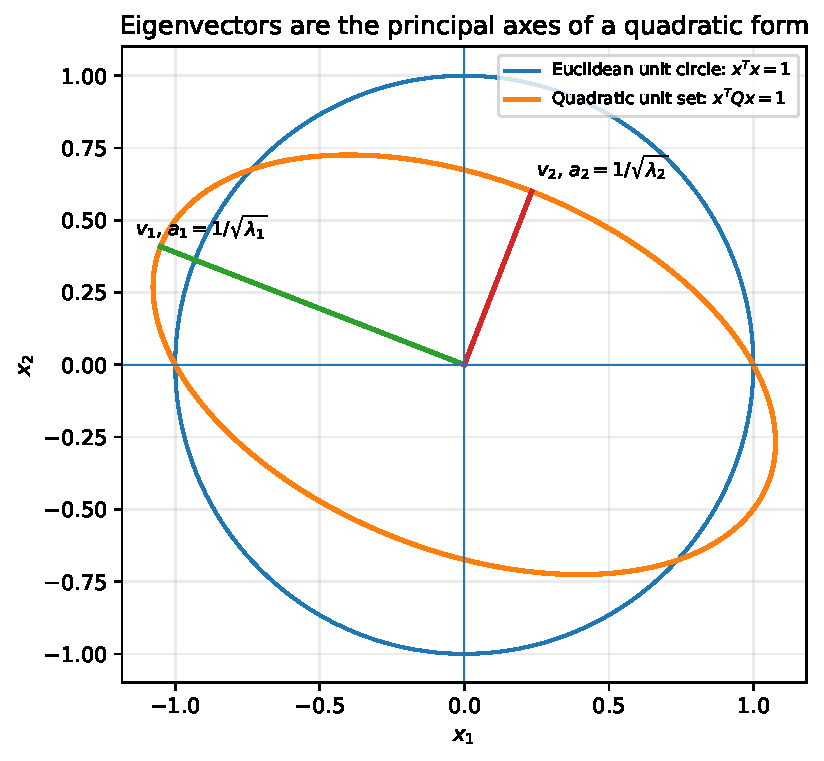
\includegraphics[width=0.72\textwidth]{figures/quadratic_form_axes.pdf}
  \caption{A positive-definite quadratic form defines an ellipse. Eigenvectors are the directions in which the form decouples, and the semi-axis along $\vct v_i$ is proportional to $1/\sqrt{\lambda_i}$.}
  \label{fig:quadratic-axes}
\end{figure}

\subsection{What positive definiteness means geometrically}

A symmetric matrix $\mat Q$ is positive definite if
\begin{equation}
  \vct x^\T\mat Q\vct x>0
  \qquad\text{for all }\vct x\neq\vct 0.
\end{equation}
Equivalently, all eigenvalues are positive.

Geometrically, positive definiteness means that every direction costs positive quadratic ``distance''. No direction is free and no direction contributes negative curvature. Therefore the level set $\vct x^\T\mat Q\vct x=c>0$ is closed and bounded: an ellipse in 2D, an ellipsoid in 3D.

If one eigenvalue is zero, motion along the associated eigenvector costs nothing. The level set then extends infinitely in that direction and becomes a cylinder. This distinction will become central for the EESM voltage limit.

\subsection{Determinants, discriminants and a common source of confusion}

For
\begin{equation}
  \mat Q=
  \begin{bmatrix}a&b\\b&c_q\end{bmatrix},
\end{equation}
the determinant is
\begin{equation}
  \det\mat Q = ac_q-b^2 = \lambda_1\lambda_2.
\end{equation}
If $\mat Q$ is positive definite, then both eigenvalues are positive, so
\begin{equation}
  \det\mat Q>0.
\end{equation}

However, a general conic is often written as
\begin{equation}
  A x^2+Bxy+Cy^2+Dx+Ey+F=0.
  \label{eq:general-conic}
\end{equation}
The quadratic-part matrix is
\begin{equation}
  \mat Q=
  \begin{bmatrix}
  A&B/2\\B/2&C
  \end{bmatrix}.
\end{equation}
The familiar conic discriminant is
\begin{equation}
  \Delta_{\mathrm{conic}}=B^2-4AC.
\end{equation}
But
\begin{equation}
  B^2-4AC = -4\det\mat Q.
  \label{eq:conic-disc-det}
\end{equation}
Therefore a positive-definite quadratic part has $\det\mat Q>0$ but \emph{negative conic discriminant}. These are not contradictory statements; they refer to two different quantities.

There is a third determinant that also appears in textbooks: the determinant of the homogeneous $3\times3$ conic matrix. For a centered ellipse
\begin{equation}
  \vct x^\T\mat Q\vct x-U^2=0,
\end{equation}
the homogeneous matrix is
\begin{equation}
  \mat C=
  \begin{bmatrix}
  \mat Q&\vct 0\\
  \vct 0^\T&-U^2
  \end{bmatrix},
\end{equation}
and hence
\begin{equation}
  \det\mat C=-U^2\det\mat Q<0.
\end{equation}
So the statements ``$\det\mat Q>0$'', ``$B^2-4AC<0$'' and ``$\det\mat C<0$'' can all be true for the same real ellipse.

\paragraph{Interpretation of the determinant.}
The determinant is the product of eigenvalues. It measures how strongly the quadratic form acts collectively across independent directions. It is also related to area scaling: for a 2D ellipse $\vct x^\T\mat Q\vct x\le c$, the area is proportional to $1/\sqrt{\det\mat Q}$. A large determinant means a small ellipse.

\subsection{Why the ellipse is rotated and where the angle formula comes from}

Write
\begin{equation}
  q(x,y)=a x^2+2bxy+c_q y^2.
\end{equation}
Rotate coordinates by an angle $\theta$,
\begin{equation}
  \begin{bmatrix}x\\y\end{bmatrix}
  =
  \begin{bmatrix}
  \cos\theta&-\sin\theta\\
  \sin\theta&\cos\theta
  \end{bmatrix}
  \begin{bmatrix}\xi\\\eta\end{bmatrix}.
\end{equation}
After substitution, the coefficient of the mixed term $\xi\eta$ is proportional to
\begin{equation}
  2b\cos(2\theta)+(c_q-a)\sin(2\theta).
\end{equation}
The principal-axis rotation is the angle that makes this mixed term vanish:
\begin{equation}
  \tan(2\theta)=\frac{2b}{a-c_q}.
  \label{eq:rotation-angle-general}
\end{equation}
The angle is defined modulo $90^\circ$ because an ellipse has two perpendicular principal axes. In numerical work, eigenvectors are usually safer than manually choosing a branch of the half-angle formula.

\paragraph{Meaning of the cross term.}
A nonzero $xy$ term says that moving in $x$ changes the cost associated with $y$ and vice versa. The original coordinate axes are therefore not the natural independent directions. Rotation into the eigenbasis removes that coupling.

\subsection{The singular-value decomposition: the most physical viewpoint}

Suppose a linear map sends current-space displacement $\vct x$ to voltage $\vct u$:
\begin{equation}
  \vct u=\mat A\vct x.
\end{equation}
A voltage circle $\|\vct u\|=U$ pulls back to
\begin{equation}
  \|\mat A\vct x\|^2
  =\vct x^\T\mat A^\T\mat A\vct x
  =U^2.
\end{equation}
Let
\begin{equation}
  \mat A=\mat U\mat\Sigma\mat V^\T
\end{equation}
be the singular-value decomposition (SVD). Then
\begin{equation}
  \mat A^\T\mat A
  =\mat V\mat\Sigma^\T\mat\Sigma\mat V^\T.
\end{equation}
Thus the right singular vectors of $\mat A$ are the current-space ellipse axes, and the eigenvalues of $\mat A^\T\mat A$ are the squared singular values:
\begin{equation}
  \lambda_i=\sigma_i^2.
\end{equation}
The semi-axis lengths are therefore
\begin{equation}
  a_i=\frac{U}{\sigma_i}.
  \label{eq:svd-axis}
\end{equation}

\paragraph{Physical analogy.}
Imagine the machine equations as a gearbox between current space and voltage space. A singular value $\sigma_i$ tells how much voltage is produced by one unit of current displacement in a special direction. A large $\sigma_i$ means the machine converts current displacement strongly into voltage, so the allowable current distance before hitting $U_{\max}$ is small. Hence the inverse relation $a_i=U_{\max}/\sigma_i$.

\section{PMSM/IPMSM: torque hyperbolas and the voltage ellipse}

\subsection{Steady-state model and conventions}

For a sinusoidal synchronous machine in steady state, neglecting dynamic derivative terms in the rotating $dq$ frame, use
\begin{align}
  u_d &= \Rs\id-\w\Lq\iq,\\
  u_q &= \Rs\iq+\w(\psipm+\Ld\id).
  \label{eq:psm-voltage}
\end{align}
Here $\omega$ is electrical angular speed. The electromagnetic torque is
\begin{equation}
  M=\frac{3}{2}p\left[\psipm\iq+(\Ld-\Lq)\id\iq\right].
  \label{eq:psm-torque}
\end{equation}
Define the saliency difference
\begin{equation}
  \Delta L=\Ld-\Lq.
\end{equation}
Then
\begin{equation}
  M=k_M\iq(\psipm+\Delta L\id),
  \qquad k_M=\frac{3}{2}p.
  \label{eq:psm-torque-factor}
\end{equation}

\subsection{Why constant-torque curves are hyperbolas}

For a prescribed torque $M^*$,
\begin{equation}
  \iq(\psipm+\Delta L\id)=\frac{M^*}{k_M}.
\end{equation}
If $\Delta L\neq0$,
\begin{equation}
  \iq=\frac{M^*/k_M}{\psipm+\Delta L\id}.
  \label{eq:torque-hyperbola}
\end{equation}
This is a shifted hyperbola with asymptotes
\begin{equation}
  \iq=0,
  \qquad
  \id=-\frac{\psipm}{\Delta L}.
\end{equation}

Two important special cases prevent overgeneralization:

\begin{itemize}
  \item If $\Delta L=0$ (surface-PM machine with $L_d=L_q$), then
  \begin{equation}
    M=k_M\psipm\iq,
  \end{equation}
  and constant-torque curves are horizontal lines, not hyperbolas.
  \item If $\psipm=0$ (pure reluctance term), then
  \begin{equation}
    M=k_M\Delta L\id\iq,
  \end{equation}
  so the hyperbolas are centered at the origin.
\end{itemize}

\paragraph{Geometric meaning.}
Torque is the product of $\iq$ and an effective $d$-axis flux term $\psipm+\Delta L\id$. Constant product gives hyperbolic geometry for exactly the same reason that $xy=c$ is a rectangular hyperbola.

\subsection{Writing the voltage equations as an affine map}

Let
\begin{equation}
  \vct i=\begin{bmatrix}\id\\\iq\end{bmatrix},
  \qquad
  \vct u=\begin{bmatrix}u_d\\u_q\end{bmatrix}.
\end{equation}
Then \eqref{eq:psm-voltage} becomes
\begin{equation}
  \vct u=\mat A\vct i+\vct b,
  \label{eq:psm-affine}
\end{equation}
with
\begin{equation}
  \mat A=
  \begin{bmatrix}
  \Rs&-\w\Lq\\
  \w\Ld&\Rs
  \end{bmatrix},
  \qquad
  \vct b=
  \begin{bmatrix}
  0\\\w\psipm
  \end{bmatrix}.
  \label{eq:psm-A-b}
\end{equation}

The inverter voltage limit is the circle
\begin{equation}
  u_d^2+u_q^2=\Umax^2
  \quad\Longleftrightarrow\quad
  \|\vct u\|=\Umax.
  \label{eq:voltage-circle}
\end{equation}
The current-space voltage limit is therefore the inverse image of a circle under the affine machine map \eqref{eq:psm-affine}.

\subsection{The ellipse center}

The center is the current point $\vct i_c$ that maps to the center of the voltage circle, $\vct u=\vct 0$:
\begin{equation}
  \mat A\vct i_c+\vct b=\vct0.
\end{equation}
If $\mat A$ is invertible,
\begin{equation}
  \vct i_c=-\mat A^{-1}\vct b.
\end{equation}
Its determinant is
\begin{equation}
  \det\mat A=\Rs^2+\w^2\Ld\Lq.
  \label{eq:detA-psm}
\end{equation}
For positive inductances, this is positive except in the idealized simultaneous case $\Rs=0$ and $\omega=0$.

The inverse is
\begin{equation}
  \mat A^{-1}
  =\frac{1}{\Rs^2+\w^2\Ld\Lq}
  \begin{bmatrix}
    \Rs&\w\Lq\\
    -\w\Ld&\Rs
  \end{bmatrix}.
\end{equation}
Therefore
\begin{align}
  i_{d,c}
  &= -\frac{\psipm\w^2\Lq}{\Rs^2+\w^2\Ld\Lq},
  \label{eq:psm-center-d}\\
  i_{q,c}
  &= -\frac{\psipm\Rs\w}{\Rs^2+\w^2\Ld\Lq}.
  \label{eq:psm-center-q}
\end{align}

At high speed,
\begin{equation}
  \lim_{|\w|\to\infty}i_{d,c}
  =-\frac{\psipm}{\Ld},
  \qquad
  \lim_{|\w|\to\infty}i_{q,c}=0.
  \label{eq:center-high-speed}
\end{equation}
This limiting point is physically meaningful: $\Ld\id+\psipm=0$ cancels the PM flux in the $q$-axis back-EMF term.

At low speed with $\Rs>0$,
\begin{equation}
  \lim_{\w\to0}\vct i_c=\vct 0.
\end{equation}
The resistive voltage drop dominates and the voltage limit approaches a current-centered circle.

\subsection{The centered quadratic form}

Define the displacement from the center
\begin{equation}
  \vct y=\vct i-\vct i_c.
\end{equation}
Since $\mat A\vct i_c+\vct b=0$,
\begin{equation}
  \vct u=\mat A\vct y.
\end{equation}
Therefore
\begin{equation}
  \|\vct u\|^2
  =\vct y^\T\mat A^\T\mat A\vct y.
\end{equation}
Define
\begin{equation}
  \mat Q=\mat A^\T\mat A.
\end{equation}
Then the voltage boundary is
\begin{equation}
  \boxed{\vct y^\T\mat Q\vct y=\Umax^2.}
  \label{eq:psm-ellipse-q}
\end{equation}
Explicitly,
\begin{equation}
  \mat Q=
  \begin{bmatrix}
  \Rs^2+\w^2\Ld^2 & \Rs\w(\Ld-\Lq)\\
  \Rs\w(\Ld-\Lq) & \Rs^2+\w^2\Lq^2
  \end{bmatrix}.
  \label{eq:psm-Q}
\end{equation}

Because $\mat Q=\mat A^\T\mat A$,
\begin{equation}
  \vct y^\T\mat Q\vct y=\|\mat A\vct y\|^2\ge0.
\end{equation}
When $\mat A$ is invertible, the equality can hold only for $\vct y=0$, so $\mat Q$ is positive definite. Thus the voltage boundary is necessarily an ellipse.

Moreover,
\begin{equation}
  \det\mat Q=(\det\mat A)^2
  =(\Rs^2+\w^2\Ld\Lq)^2>0.
  \label{eq:detQ-psm}
\end{equation}
This single identity gives several pieces of information at once: invertibility of the current-to-voltage map, positive area scaling, and a negative conic discriminant through \eqref{eq:conic-disc-det}.

\subsection{Principal axes and semi-axis lengths}

Let $\lambda_1,\lambda_2$ be the eigenvalues of $\mat Q$, with orthonormal eigenvectors $\vct v_1,\vct v_2$. In principal coordinates $z_i=\vct v_i^\T\vct y$,
\begin{equation}
  \lambda_1 z_1^2+\lambda_2 z_2^2=\Umax^2.
\end{equation}
Hence
\begin{equation}
  a_i=\frac{\Umax}{\sqrt{\lambda_i}}.
  \label{eq:psm-axis-eigen}
\end{equation}
The long axis corresponds to the smaller eigenvalue.

Equivalently, if $\sigma_i$ are the singular values of $\mat A$,
\begin{equation}
  a_i=\frac{\Umax}{\sigma_i}.
\end{equation}
This is often the cleanest physical interpretation: the ellipse is large in current directions that create little voltage and small in directions that create voltage efficiently.

\subsection{The rotation angle for the PMSM ellipse}

Using \eqref{eq:rotation-angle-general} with the entries of \eqref{eq:psm-Q},
\begin{equation}
  \tan(2\theta)
  =\frac{2\Rs\w(\Ld-\Lq)}{\w^2(\Ld^2-\Lq^2)}.
\end{equation}
For $\Ld\neq\Lq$ this simplifies to
\begin{equation}
  \boxed{
  \tan(2\theta)=\frac{2\Rs}{\w(\Ld+\Lq)}.
  }
  \label{eq:psm-angle}
\end{equation}
The formula determines the principal-axis orientation modulo $90^\circ$.

Several limits are worth understanding rather than memorizing:

\begin{itemize}
  \item If $\Rs=0$, then $\theta=0$: the ideal voltage ellipse is aligned with the $dq$ axes.
  \item If $|\w|\to\infty$, then $\theta\to0$: inductive voltage dominates resistance, so the axes realign with $d$ and $q$.
  \item If $\w\to0$ while $\Rs>0$, then $\mat Q\to\Rs^2\mat I$. The ellipse becomes a circle, so its orientation is physically undefined. A half-angle formula may return a limiting numerical angle, but that angle has no geometric significance when both eigenvalues are equal.
  \item Reversing $\w$ reverses the sign of the cross term and therefore mirrors the tilt.
\end{itemize}

\subsection{The ideal ellipse as the familiar textbook formula}

Setting $\Rs=0$ in \eqref{eq:psm-voltage} gives
\begin{align}
  u_d&=-\w\Lq\iq,\\
  u_q&=\w(\psipm+\Ld\id).
\end{align}
Thus
\begin{equation}
  \Lq^2\iq^2+(\psipm+\Ld\id)^2
  =\left(\frac{\Umax}{|\w|}\right)^2.
  \label{eq:ideal-voltage-ellipse}
\end{equation}
The center is fixed at
\begin{equation}
  \left(-\frac{\psipm}{\Ld},0\right),
\end{equation}
and the semi-axes are
\begin{equation}
  a_d=\frac{\Umax}{|\w|\Ld},
  \qquad
  a_q=\frac{\Umax}{|\w|\Lq}.
  \label{eq:ideal-axes}
\end{equation}
Both shrink as $1/|\omega|$. This is the simplest geometric picture of field weakening: increasing speed tightens the admissible voltage ellipse around its flux-cancellation center.

\begin{figure}[htbp]
  \centering
  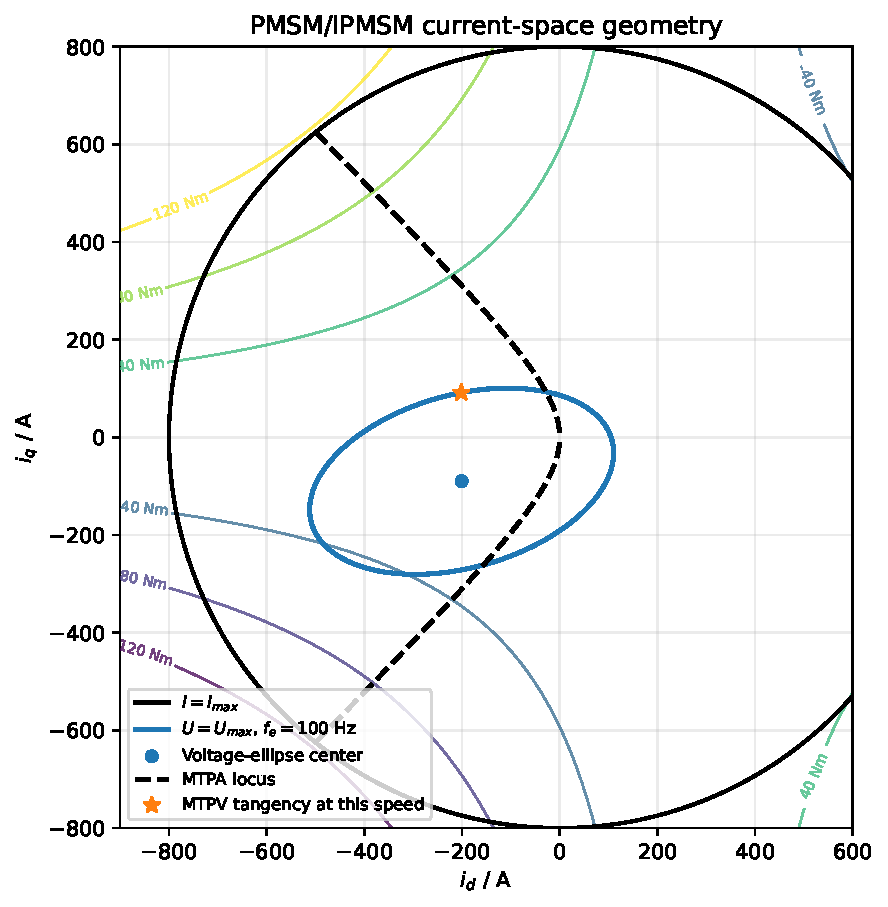
\includegraphics[width=0.82\textwidth]{figures/psm_geometry.pdf}
  \caption{Representative PMSM/IPMSM current-space geometry. The torque contours, current limit and voltage ellipse live in the same $(i_d,i_q)$ plane. MTPA is a tangency with a current-magnitude contour; MTPV is a tangency with the voltage ellipse when the current constraint is inactive.}
  \label{fig:psm-geometry}
\end{figure}

\section{MTPA, field weakening and MTPV as tangency problems}

\subsection{Why constrained optima are tangent}

Suppose one minimizes a function $f(\vct x)$ subject to one equality $g(\vct x)=0$. Along the constraint, allowed infinitesimal motions $d\vct x$ satisfy
\begin{equation}
  \nabla g^\T d\vct x=0.
\end{equation}
At a constrained optimum, the objective cannot change to first order along any allowed tangent direction:
\begin{equation}
  \nabla f^\T d\vct x=0.
\end{equation}
Therefore both $\nabla f$ and $\nabla g$ are normals to the same tangent space, so they must be parallel:
\begin{equation}
  \nabla f=\lambda\nabla g.
  \label{eq:lagrange-geometric}
\end{equation}
This is the geometric content of the Lagrange multiplier.

\begin{figure}[htbp]
  \centering
  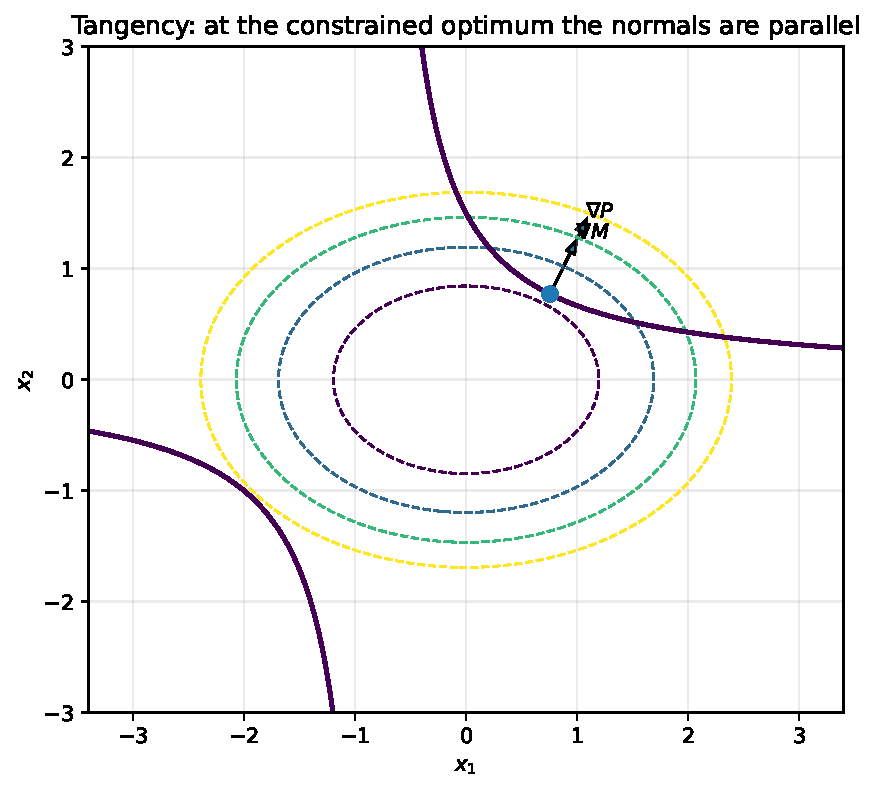
\includegraphics[width=0.66\textwidth]{figures/tangency_gradients.pdf}
  \caption{At a constrained optimum, the objective level set and constraint are tangent. Their gradients are normal to the same tangent direction and are therefore parallel.}
  \label{fig:tangency}
\end{figure}

\subsection{PMSM MTPA: minimum current for a required torque}

Define
\begin{equation}
  I^2=\id^2+\iq^2.
\end{equation}
For a prescribed torque $M^*$, MTPA solves
\begin{equation}
  \min_{\id,\iq} I^2
  \qquad\text{subject to}\qquad
  M(\id,\iq)=M^*.
  \label{eq:mtpa-problem}
\end{equation}
The gradients are
\begin{equation}
  \nabla I^2=
  \begin{bmatrix}2\id\\2\iq\end{bmatrix},
\end{equation}
and, using \eqref{eq:psm-torque-factor},
\begin{equation}
  \nabla M
  =k_M
  \begin{bmatrix}
  \Delta L\iq\\
  \psipm+\Delta L\id
  \end{bmatrix}.
\end{equation}
Tangency requires the two vectors to be parallel. In two dimensions, parallelism is equivalent to a zero determinant (or scalar cross product):
\begin{equation}
  \det
  \begin{bmatrix}
  2\id & \Delta L\iq\\
  2\iq & \psipm+\Delta L\id
  \end{bmatrix}=0.
\end{equation}
After simplification,
\begin{equation}
  \boxed{
  \psipm\id+\Delta L(\id^2-\iq^2)=0.
  }
  \label{eq:mtpa-locus}
\end{equation}
This is the MTPA locus.

For $\Delta L\neq0$, one explicit branch is
\begin{equation}
  \id=\frac{-\psipm+\sqrt{\psipm^2+4\Delta L^2\iq^2}}{2\Delta L},
  \label{eq:mtpa-explicit}
\end{equation}
where the branch is chosen so that $\id\to0$ as $\iq\to0$. For the common IPMSM case $\Lq>\Ld$, hence $\Delta L<0$, positive-torque MTPA uses negative $i_d$.

For a surface-PM machine with $\Delta L=0$, \eqref{eq:mtpa-locus} reduces to
\begin{equation}
  \psipm\id=0,
\end{equation}
so MTPA is simply $\id=0$.

\paragraph{Geometric analogy.}
Imagine circles of increasing radius centered at the origin. The first circle that touches a chosen torque hyperbola does so tangentially. That first touch is the smallest current magnitude capable of producing the requested torque.

\subsection{PMSM MTPV: maximum torque on the voltage boundary}

When the current limit is inactive and the voltage limit is active, one solves
\begin{equation}
  \max_{\vct i} M(\vct i)
  \qquad\text{subject to}\qquad
  g_U(\vct i)=\|\vct u(\vct i)\|^2-\Umax^2=0.
  \label{eq:mtpv-problem}
\end{equation}
From the centered form \eqref{eq:psm-ellipse-q},
\begin{equation}
  g_U=(\vct i-\vct i_c)^\T\mat Q(\vct i-\vct i_c)-\Umax^2,
\end{equation}
and therefore
\begin{equation}
  \nabla g_U=2\mat Q(\vct i-\vct i_c).
  \label{eq:grad-voltage-q}
\end{equation}
The MTPV condition is
\begin{equation}
  \boxed{
  \nabla M=\mu\,2\mat Q(\vct i-\vct i_c).
  }
  \label{eq:mtpv-general}
\end{equation}
In words: a torque contour is tangent to the voltage ellipse.

For the ideal case $\Rs=0$, use
\begin{equation}
  h(\id,\iq)=\Lq^2\iq^2+(\psipm+\Ld\id)^2.
\end{equation}
The speed-dependent factor $\omega^2$ multiplies the whole voltage expression and therefore cancels from the tangency condition. Computing the two gradients and setting their 2D cross product to zero gives
\begin{equation}
  \boxed{
  \Delta L\Lq^2\iq^2
  =\Ld(\psipm+\Delta L\id)(\psipm+\Ld\id).
  }
  \label{eq:ideal-mtpv-locus}
\end{equation}
Thus the ideal machine has a speed-independent MTPV \emph{locus}; different voltage ellipses touch that same locus at different points.

With $\Rs\neq0$, both $\mat Q$ and the center $\vct i_c$ vary with speed, so there is generally no single speed-independent MTPV curve.

\subsection{The three classical active-constraint regions}

At a fixed speed, maximum torque with both current and voltage limits can be written
\begin{equation}
  \max M(\vct i)
\end{equation}
subject to
\begin{align}
  g_I(\vct i)&=\id^2+\iq^2-\Imax^2\le0,\\
  g_U(\vct i)&=\|\vct u\|^2-\Umax^2\le0.
\end{align}
The KKT stationarity condition has the form
\begin{equation}
  \nabla M
  =\lambda_I\nabla g_I+\lambda_U\nabla g_U,
  \qquad
  \lambda_I,\lambda_U\ge0.
  \label{eq:kkt-psm}
\end{equation}
Complementarity requires
\begin{equation}
  \lambda_I g_I=0,
  \qquad
  \lambda_U g_U=0.
\end{equation}
This creates three geometrically distinct regimes:

\begin{enumerate}
  \item \textbf{Current-limited region:} $\lambda_I>0$, $\lambda_U=0$. The optimum is a torque contour tangent to the current circle, i.e. the full-current MTPA point.
  \item \textbf{Mixed field-weakening region:} $\lambda_I>0$, $\lambda_U>0$. Both current circle and voltage ellipse are active. The optimum lies at their intersection; a torque contour need not be tangent to either one individually because both constraint normals participate in \eqref{eq:kkt-psm}.
  \item \textbf{Voltage-limited region:} $\lambda_I=0$, $\lambda_U>0$. The torque contour is tangent to the voltage ellipse, i.e. MTPV.
\end{enumerate}

This is the rigorous reason that ``MTPA $\rightarrow$ intersection $\rightarrow$ MTPV'' is a natural geometric progression as speed increases.

\section{A numerical PMSM example}

Consider the illustrative parameters
\begin{equation}
\Rs=\SI{90}{m\ohm},\quad
\Ld=\SI{160}{\micro\henry},\quad
\Lq=\SI{320}{\micro\henry},\quad
\psipm=\SI{45}{m\weber},\quad
\Umax=\SI{40}{V}.
\end{equation}
Then
\begin{equation}
  -\frac{\psipm}{\Ld}=-281.25\ \mathrm{A}.
\end{equation}
This is the high-speed limiting center of the voltage ellipse.

Table \ref{tab:psm-numeric} shows how the center, long semi-axis and principal-axis angle evolve with speed. The long-axis angle is obtained from the eigenvector associated with the smaller eigenvalue of $\mat Q$.

\begin{table}[htbp]
\centering
\caption{Illustrative PMSM voltage-ellipse geometry for $\Umax=\SI{40}{V}$.}
\label{tab:psm-numeric}
\begin{tabular}{rrrrr}
\toprule
$f_e$ / Hz & $i_{d,c}$ / A & $i_{q,c}$ / A & long semi-axis / A & long-axis angle / deg\\
\midrule
50   & -108.1 & -96.7 & 433.5 & 25.0\\
100  & -200.8 & -89.9 & 319.1 & 15.4\\
250  & -264.3 & -47.3 & 152.7 & 6.7\\
500  & -276.8 & -24.8 & 78.7  & 3.4\\
1000 & -280.1 & -12.5 & 39.7  & 1.7\\
1500 & -280.7 & -8.4  & 26.5  & 1.1\\
\bottomrule
\end{tabular}
\end{table}

The table makes three effects visible:

\begin{itemize}
  \item the center approaches $(-\psipm/\Ld,0)$,
  \item the ellipse shrinks approximately as $1/|\omega|$ once inductive voltage dominates,
  \item the resistance-induced tilt disappears at high speed.
\end{itemize}

\section{EESM: the same geometry lifted into three dimensions}

\subsection{Linear EESM model}

Introduce excitation current $\ie$ and the linear excitation-flux model
\begin{equation}
  \psi_{\mathrm{exc}}=\Lexc\ie.
  \label{eq:eesm-flux}
\end{equation}
The steady-state stator voltage equations become
\begin{align}
  u_d &= \Rs\id-\w\Lq\iq,\\
  u_q &= \Rs\iq+\w(\Ld\id+\Lexc\ie).
  \label{eq:eesm-voltage}
\end{align}
Torque is
\begin{equation}
  \boxed{
  M=k_M\iq(\Lexc\ie+\Delta L\id).
  }
  \label{eq:eesm-torque}
\end{equation}
The natural current-space coordinate is now
\begin{equation}
  \vct x=\begin{bmatrix}\id\\\iq\\\ie\end{bmatrix}\in\R^3.
\end{equation}

\subsection{Fixed-excitation slices: every slice is a PMSM-like ellipse}

Hold $\ie$ fixed. Then the EESM stator-voltage equations have exactly the same form as the PMSM equations, with
\begin{equation}
  \psipm\quad\longrightarrow\quad\Lexc\ie.
\end{equation}
Therefore each plane $\ie=\text{constant}$ contains a voltage ellipse with the same $2\times2$ shape matrix \eqref{eq:psm-Q}. Only its center changes:
\begin{align}
  i_{d,c}(\ie)
  &= -\frac{\Lexc\ie\,\w^2\Lq}{\Rs^2+\w^2\Ld\Lq},\\
  i_{q,c}(\ie)
  &= -\frac{\Lexc\ie\,\Rs\w}{\Rs^2+\w^2\Ld\Lq}.
  \label{eq:eesm-slice-center}
\end{align}
Both coordinates depend linearly on $\ie$.

This gives an immediate geometric picture: \emph{stack congruent ellipses while their centers move along a straight line}. The result is an oblique elliptic cylinder.

\begin{figure}[htbp]
  \centering
  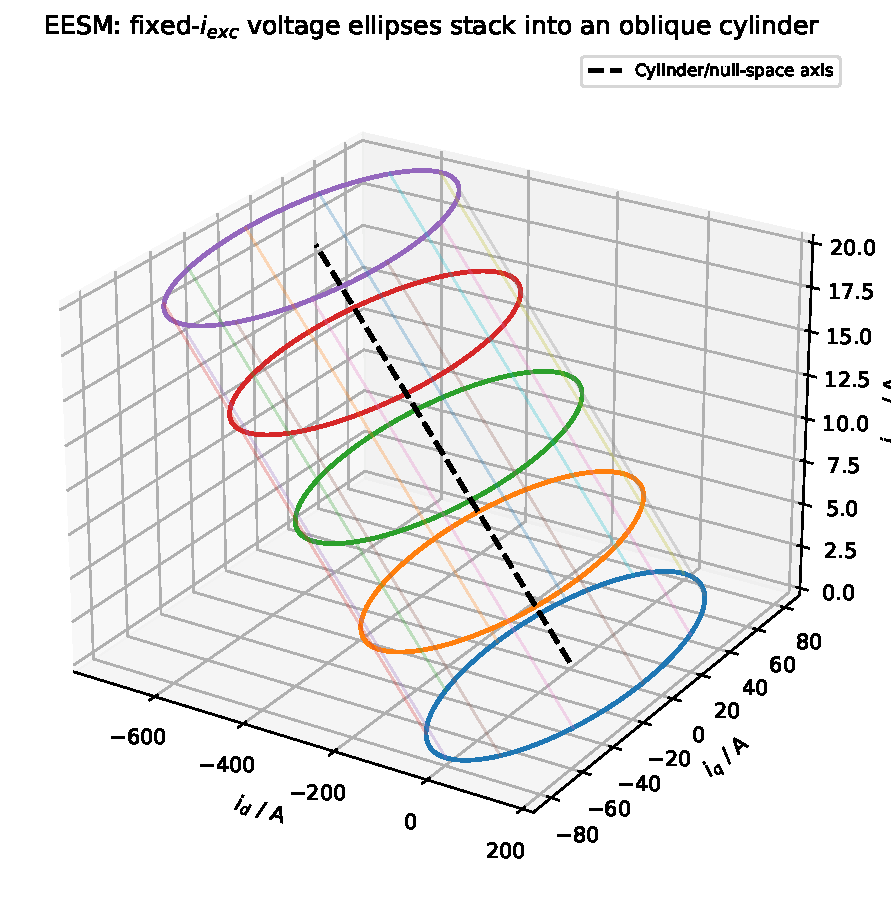
\includegraphics[width=0.86\textwidth]{figures/eesm_voltage_cylinder_slices.pdf}
  \caption{In the EESM, each fixed-$i_{\mathrm{exc}}$ slice is a PMSM-like voltage ellipse. Because the ellipse shape is unchanged while its center moves linearly with excitation current, the stacked surface is an oblique elliptic cylinder. The ideal case is shown for clarity.}
  \label{fig:eesm-slices}
\end{figure}

\subsection{Matrix proof: why the EESM voltage surface is a cylinder, not an ellipsoid}

Write \eqref{eq:eesm-voltage} as
\begin{equation}
  \vct u=\mat A_E\vct x,
\end{equation}
with
\begin{equation}
  \mat A_E=
  \begin{bmatrix}
  \Rs&-\w\Lq&0\\
  \w\Ld&\Rs&\w\Lexc
  \end{bmatrix}
  \in\R^{2\times3}.
  \label{eq:eesm-A}
\end{equation}
The voltage boundary is
\begin{equation}
  \vct x^\T\mat Q_U\vct x=\Umax^2,
  \qquad
  \mat Q_U=\mat A_E^\T\mat A_E.
  \label{eq:eesm-voltage-q}
\end{equation}
Explicitly,
\begin{equation}
\mat Q_U=
\begin{bmatrix}
\Rs^2+\w^2\Ld^2 & \Rs\w(\Ld-\Lq) & \w^2\Ld\Lexc\\
\Rs\w(\Ld-\Lq) & \Rs^2+\w^2\Lq^2 & \Rs\w\Lexc\\
\w^2\Ld\Lexc & \Rs\w\Lexc & \w^2\Lexc^2
\end{bmatrix}.
\label{eq:eesm-QU-explicit}
\end{equation}

The decisive observation is not the individual entries but the dimensions of $\mat A_E$. A $2\times3$ matrix has rank at most 2. Hence
\begin{equation}
  \operatorname{rank}(\mat Q_U)
  =\operatorname{rank}(\mat A_E)\le2.
\end{equation}
For the nondegenerate machine and nonzero speed, the rank is normally exactly 2. Therefore $\mat Q_U$ has two positive eigenvalues and one zero eigenvalue:
\begin{equation}
  \lambda_1>0,\qquad\lambda_2>0,\qquad\lambda_3=0.
\end{equation}
In principal coordinates,
\begin{equation}
  \lambda_1z_1^2+\lambda_2z_2^2+0\cdot z_3^2=\Umax^2.
  \label{eq:eesm-cylinder-principal}
\end{equation}
The coordinate $z_3$ is unrestricted. Equation \eqref{eq:eesm-cylinder-principal} is exactly an elliptic cylinder.

\paragraph{Why ``$i_{exc}$ appears in $u_q$'' does not close the surface.}
It is tempting to think that dependence on all three currents must produce a closed 3D ellipsoid. The missing piece is the number of independent output constraints. There are only two stator-voltage components, $u_d$ and $u_q$. Three current coordinates are mapped into a two-dimensional voltage vector, so one current-space direction must remain invisible to the voltage norm. That invisible direction is the cylinder axis.

\subsection{The null-space direction: the cylinder axis}

A cylinder-axis direction $\vct n\neq0$ satisfies
\begin{equation}
  \mat A_E\vct n=0.
  \label{eq:nullspace-axis}
\end{equation}
Then
\begin{equation}
  \vct u(\vct x+t\vct n)
  =\mat A_E\vct x+t\mat A_E\vct n
  =\vct u(\vct x)
\end{equation}
for every scalar $t$. Moving along $\vct n$ leaves stator voltage unchanged.

For $\Rs\neq0$, choose $n_q$ freely. The first row gives
\begin{equation}
  n_d=\frac{\w\Lq}{\Rs}n_q,
\end{equation}
and the second gives
\begin{equation}
  n_{\mathrm{exc}}
  =-\frac{\Rs^2+\w^2\Ld\Lq}{\Rs\w\Lexc}n_q.
  \label{eq:eesm-null-vector}
\end{equation}

In the ideal case $\Rs=0$, the equations simplify dramatically:
\begin{equation}
  \iq=0,
  \qquad
  \Ld\id+\Lexc\ie=0.
\end{equation}
One convenient axis vector is therefore
\begin{equation}
  \boxed{
  \vct n=
  \begin{bmatrix}
  -\Lexc/\Ld\\0\\1
  \end{bmatrix}.
  }
  \label{eq:ideal-eesm-null}
\end{equation}
This is exactly the line traced by the centers of the fixed-excitation voltage ellipses.

\subsection{SVD interpretation in 3D}

The SVD of $\mat A_E\in\R^{2\times3}$ has two nonzero singular values $\sigma_1,\sigma_2$ and one zero singular value. In the right-singular-vector coordinates,
\begin{equation}
  \sigma_1^2z_1^2+\sigma_2^2z_2^2=\Umax^2,
\end{equation}
while $z_3$ is free. Therefore
\begin{equation}
  a_1=\frac{\Umax}{\sigma_1},
  \qquad
  a_2=\frac{\Umax}{\sigma_2},
  \qquad
  a_3=\infty.
\end{equation}
This is perhaps the cleanest single-line explanation of the EESM voltage cylinder.

\section{EESM torque surfaces and copper-loss ellipsoids}

\subsection{Torque surfaces are hyperbolic cylinders in transformed coordinates}

The EESM torque equation is
\begin{equation}
  M=k_M\iq(\Lexc\ie+\Delta L\id).
\end{equation}
Introduce the linear coordinate
\begin{equation}
  s=\Lexc\ie+\Delta L\id.
\end{equation}
Then
\begin{equation}
  M=k_M\iq s.
\end{equation}
For $M^*\neq0$,
\begin{equation}
  \iq s=\frac{M^*}{k_M},
\end{equation}
which is a hyperbola in the $(s,\iq)$ plane. A third independent coordinate can move along directions satisfying
\begin{equation}
  \Delta L\,\delta i_d+\Lexc\,\delta i_{\mathrm{exc}}=0
\end{equation}
without changing $s$, and therefore without changing torque. Thus a constant-torque set is a hyperbolic cylinder in an appropriate rotated/sheared coordinate system.

For $M=0$, the surface degenerates into the union
\begin{equation}
  \iq=0
  \qquad\text{or}\qquad
  \Lexc\ie+\Delta L\id=0.
\end{equation}

\paragraph{Interpretation.}
The EESM adds a second way to create the flux factor multiplying $i_q$: either through field current $i_{\mathrm{exc}}$ or through reluctance contribution $\Delta L i_d$. Torque depends only on their weighted sum. This redundancy is why torque level sets extend in a third direction.

\subsection{Copper loss is a genuine ellipsoid}

Use the copper-loss model
\begin{equation}
  P_{\mathrm{Cu}}
  =\Rexc\ie^2+\frac{3}{2}\Rs(\id^2+\iq^2).
  \label{eq:eesm-pcu}
\end{equation}
Define
\begin{equation}
  \mat R=
  \operatorname{diag}\left(
  \frac{3}{2}\Rs,
  \frac{3}{2}\Rs,
  \Rexc
  \right).
\end{equation}
Then
\begin{equation}
  P_{\mathrm{Cu}}=\vct x^\T\mat R\vct x.
\end{equation}
If $\Rs>0$ and $\Rexc>0$, then $\mat R$ is positive definite. Therefore
\begin{equation}
  \boxed{
  \vct x^\T\mat R\vct x=\Pmax
  }
  \label{eq:loss-ellipsoid}
\end{equation}
is a closed ellipsoid.

Its principal axes are already aligned with $(i_d,i_q,i_{\mathrm{exc}})$ because $\mat R$ is diagonal. The semi-axes are
\begin{align}
  a_d=a_q
  &=\sqrt{\frac{\Pmax}{(3/2)\Rs}},\\
  a_{\mathrm{exc}}
  &=\sqrt{\frac{\Pmax}{\Rexc}}.
  \label{eq:loss-axes}
\end{align}
If the physical excitation current is restricted to $\ie\ge0$, only the upper half of this mathematical ellipsoid is feasible.

\paragraph{Terminology.}
This surface should be called a copper-loss or thermal-budget ellipsoid, not an output-power ellipsoid. At fixed mechanical speed, maximizing torque also maximizes mechanical output power, but $P_{\mathrm{Cu}}$ itself represents dissipated copper power.

\begin{figure}[htbp]
  \centering
  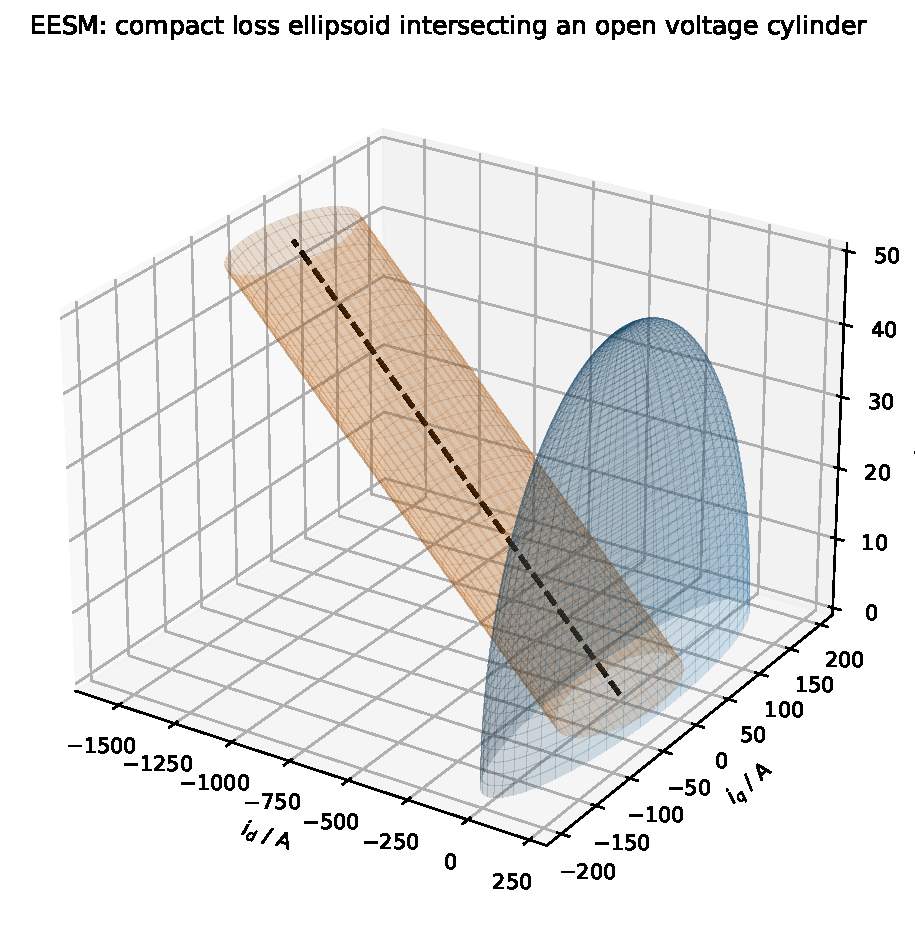
\includegraphics[width=0.86\textwidth]{figures/eesm_loss_ellipsoid_voltage_cylinder.pdf}
  \caption{The EESM copper-loss constraint is compact because its quadratic form is positive definite. The stator-voltage constraint is an open elliptic cylinder because its quadratic form is only positive semidefinite and has one zero eigenvalue. Their intersection is bounded when the loss ellipsoid is active.}
  \label{fig:eesm-loss-voltage}
\end{figure}

\section{EESM minimum-loss operation: the MTPA analogue}

\subsection{Optimization statement}

With an independent excitation winding, minimizing only stator current magnitude no longer measures total copper effort. A more physically meaningful problem is
\begin{equation}
  \min_{\id,\iq,\ie}P_{\mathrm{Cu}}
  \qquad\text{subject to}\qquad
  M=M^*.
  \label{eq:eesm-minloss}
\end{equation}
This may be interpreted as a minimum-copper-loss version of MTPA.

Geometrically, expand the copper-loss ellipsoid from the origin until it first touches the desired torque surface. The first contact is tangent.

\subsection{Lagrange derivation}

The loss gradient is
\begin{equation}
  \nabla P_{\mathrm{Cu}}
  =
  \begin{bmatrix}
  3\Rs\id\\
  3\Rs\iq\\
  2\Rexc\ie
  \end{bmatrix}.
  \label{eq:grad-pcu}
\end{equation}
The torque gradient is
\begin{equation}
  \nabla M
  =k_M
  \begin{bmatrix}
  \Delta L\iq\\
  \Lexc\ie+\Delta L\id\\
  \Lexc\iq
  \end{bmatrix}.
  \label{eq:grad-eesm-torque}
\end{equation}
At the optimum,
\begin{equation}
  \nabla P_{\mathrm{Cu}}=\lambda\nabla M.
  \label{eq:eesm-minloss-lagrange}
\end{equation}
Thus
\begin{align}
  3\Rs\id &= \lambda k_M\Delta L\iq,\\
  3\Rs\iq &= \lambda k_M(\Lexc\ie+\Delta L\id),\\
  2\Rexc\ie &= \lambda k_M\Lexc\iq.
  \label{eq:eesm-lagrange-components}
\end{align}
Assuming the nondegenerate positive-torque branch with $\iq\neq0$, eliminate $\lambda$ between the first and third equations:
\begin{equation}
  \boxed{
  \id
  =\frac{2\Rexc\Delta L}{3\Rs\Lexc}\ie.
  }
  \label{eq:eesm-opt-id-ie}
\end{equation}
Eliminating $\lambda$ between the second and third gives
\begin{equation}
  3\Rs\Lexc\iq^2
  =2\Rexc\ie(\Lexc\ie+\Delta L\id).
  \label{eq:eesm-opt-iq}
\end{equation}
Substituting \eqref{eq:eesm-opt-id-ie} shows that $\iq$ is also proportional to $\ie$. Therefore, in this idealized constant-parameter model, the minimum-loss current ratios are constant: the locus is a ray in three-dimensional current space.

\subsection{Why a straight ray is not an accident: homogeneity}

Both torque and copper loss are homogeneous quadratic functions:
\begin{align}
  M(\rho\vct x)&=\rho^2M(\vct x),\\
  P_{\mathrm{Cu}}(\rho\vct x)&=\rho^2P_{\mathrm{Cu}}(\vct x).
\end{align}
Scaling all currents by $\rho$ changes torque and copper loss by the same factor $\rho^2$. Consequently, the direction that gives the best torque-to-loss ratio is independent of the requested torque magnitude. Only the scale along that direction changes.

Real machines break this exact ray property through saturation, cross-saturation, temperature-dependent resistances, iron losses, converter losses and current limits. But the linear model makes the underlying geometry unusually transparent.

\subsection{Generalized eigenvalue interpretation}

The EESM torque can itself be written as a symmetric quadratic form
\begin{equation}
  M=\vct x^\T\mat H_M\vct x,
\end{equation}
with
\begin{equation}
  \mat H_M=
  \frac{k_M}{2}
  \begin{bmatrix}
  0&\Delta L&0\\
  \Delta L&0&\Lexc\\
  0&\Lexc&0
  \end{bmatrix}.
  \label{eq:HM}
\end{equation}
Maximizing torque for a fixed copper-loss budget,
\begin{equation}
  \max \vct x^\T\mat H_M\vct x
  \quad\text{subject to}\quad
  \vct x^\T\mat R\vct x=P_0,
\end{equation}
leads to
\begin{equation}
  \mat H_M\vct x=\lambda\mat R\vct x.
  \label{eq:generalized-eigen}
\end{equation}
This is a generalized eigenvalue problem.

A useful transformation is the ``loss whitening'' coordinate
\begin{equation}
  \vct y=\mat R^{1/2}\vct x.
\end{equation}
Then the loss constraint becomes the ordinary sphere $\vct y^\T\vct y=P_0$, while torque becomes
\begin{equation}
  M=\vct y^\T
  \left(\mat R^{-1/2}\mat H_M\mat R^{-1/2}\right)
  \vct y.
\end{equation}
The best direction is the eigenvector of this symmetric matrix associated with the largest eigenvalue.

\paragraph{Connection back to the first section.}
Once again, an optimization that looked machine-specific becomes an eigenvector problem after choosing the correct metric. The loss ellipsoid is turned into a sphere, and the best torque direction is a principal direction of the torque quadratic form measured in that loss metric.

\section{Why pure EESM MTPV is generally ill-posed in the simplified model}

\subsection{The tempting but incomplete problem}

A direct extension of PMSM MTPV would be
\begin{equation}
  \max_{\vct x}M(\vct x)
  \qquad\text{subject to}\qquad
  \vct x^\T\mat Q_U\vct x=\Umax^2.
  \label{eq:naive-eesm-mtpv}
\end{equation}
But the voltage surface is an infinite cylinder. A closed voltage ellipse in the PMSM became open in the EESM because $\mat Q_U$ acquired a zero eigenvalue.

\subsection{Explicit proof in the ideal case}

For $\Rs=0$, a null-space direction is
\begin{equation}
  \vct n=
  \begin{bmatrix}
  -\Lexc/\Ld\\0\\1
  \end{bmatrix}.
\end{equation}
Take any voltage-feasible point
\begin{equation}
  \vct x_0=
  \begin{bmatrix}
  i_{d0}\\i_{q0}\\i_{e0}
  \end{bmatrix}
\end{equation}
with $i_{q0}\neq0$. Every point
\begin{equation}
  \vct x(t)=\vct x_0+t\vct n
\end{equation}
has exactly the same stator voltage because $\mat A_E\vct n=0$.

The torque factor evolves as
\begin{align}
  \Lexc i_e(t)+\Delta L i_d(t)
  &=\Lexc(i_{e0}+t)
  +\Delta L\left(i_{d0}-\frac{\Lexc}{\Ld}t\right)\\
  &=\Lexc i_{e0}+\Delta L i_{d0}
  +t\Lexc\left(1-\frac{\Delta L}{\Ld}\right)\\
  &=\Lexc i_{e0}+\Delta L i_{d0}
  +t\Lexc\frac{\Lq}{\Ld}.
  \label{eq:torque-along-null}
\end{align}
Therefore
\begin{equation}
  M(t)=k_M i_{q0}
  \left[
  \Lexc i_{e0}+\Delta L i_{d0}
  +t\Lexc\frac{\Lq}{\Ld}
  \right].
\end{equation}
For suitable sign of $t$ and $i_{q0}$, the torque grows without bound while stator voltage remains unchanged. Thus \eqref{eq:naive-eesm-mtpv} does not possess a finite global maximum.

\paragraph{Important numerical consequence.}
If a simulation searches for ``MTPV'' only on a finite box
\begin{equation}
  i_d\in[i_{d,\min},i_{d,\max}],\quad
  i_q\in[i_{q,\min},i_{q,\max}],\quad
  i_{\mathrm{exc}}\in[0,i_{\mathrm{exc,max}}],
\end{equation}
then it may return a finite point merely because the computational box silently added extra constraints. Such a point can jump when the grid bounds change. This explains why seemingly strange 3D MTPV trajectories may appear in mockups.

\subsection{How to make the EESM high-speed optimization well posed}

Add at least one compact resource constraint, for example
\begin{equation}
  P_{\mathrm{Cu}}\le\Pmax,
  \label{eq:loss-bound}
\end{equation}
or explicit bounds on stator and excitation currents. A practical high-speed problem is then
\begin{equation}
  \boxed{
  \max_{\vct x}M(\vct x)
  }
\end{equation}
subject to
\begin{align}
  \vct x^\T\mat Q_U(\omega)\vct x&\le\Umax^2,\\
  \vct x^\T\mat R\vct x&\le\Pmax,\\
  0\le\ie&\le I_{\mathrm{exc,max}}
  \quad\text{if required.}
  \label{eq:eesm-practical-opt}
\end{align}
The loss ellipsoid is compact. Its intersection with the voltage cylinder is therefore bounded. Since torque is continuous, a finite maximum exists on that compact feasible set.

With only voltage and loss constraints active, the KKT stationarity condition is
\begin{equation}
  \boxed{
  \nabla M
  =\lambda_U\,2\mat Q_U\vct x
  +\lambda_P\,2\mat R\vct x.
  }
  \label{eq:eesm-kkt}
\end{equation}
This is the 3D counterpart of the PMSM mixed field-weakening condition: the torque-surface normal is a linear combination of the active constraint normals.

\paragraph{Terminology caution.}
For a PMSM, ``MTPV'' naturally means tangency to a closed voltage ellipse. For an EESM with independently variable field current, the same phrase must be interpreted with care. A meaningful finite high-speed optimum generally includes another current, excitation or loss constraint. It is often more precise to say ``maximum torque under voltage and thermal/current constraints''.

\section{Comparing the main geometric objects}

\begin{table}[htbp]
\centering
\caption{Geometry of the principal level sets in the simplified models.}
\begin{tabular}{p{0.24\textwidth}p{0.34\textwidth}p{0.32\textwidth}}
\toprule
Object & PMSM/IPMSM & EESM\\
\midrule
Torque level & Hyperbola in $(i_d,i_q)$ if $L_d\neq L_q$; line if $L_d=L_q$ & Hyperbolic-cylinder-type surface in $(i_d,i_q,i_{exc})$\\[0.4em]
Stator-voltage level & Ellipse; $Q=A^TA$ positive definite & Oblique elliptic cylinder; $Q=A_E^TA_E$ positive semidefinite, rank 2\\[0.4em]
Current/loss resource & Current circle $i_d^2+i_q^2=I^2$ & Copper-loss ellipsoid $P_{Cu}=P_0$ if total copper loss is used\\[0.4em]
MTPA concept & Smallest current circle tangent to torque contour & Smallest loss ellipsoid tangent to torque surface (minimum-copper-loss analogue)\\[0.4em]
MTPV concept & Torque contour tangent to closed voltage ellipse & Voltage-only problem generally unbounded; needs an additional compact constraint\\
\bottomrule
\end{tabular}
\end{table}

\section{Numerical geometry: Delaunay search, contours and isosurfaces}

\subsection{Why the numerical iso-level approach is conceptually valuable}

An analytic derivation is useful for understanding, but a numerical iso-level search has an important practical advantage: it does not require the machine equations to be algebraically solved for one current component. This becomes valuable when the model later contains saturation maps, cross-coupling, measured flux linkages or lookup tables.

The general pattern is
\begin{equation}
  f(\vct x)=f^*.
\end{equation}
Sample $f$ on a grid or mesh, then find where the scalar field crosses the target level $f^*$.

\subsection{Two dimensions}

In 2D, a triangulation decomposes the domain into triangles. If an edge has scalar values on opposite sides of the target level, the iso-contour crosses that edge. Interpolating those edge crossings produces samples of the contour. This is a natural way to obtain torque hyperbolas or voltage ellipses without rearranging their equations.

For visualization, MATLAB's \texttt{contour} already performs an equivalent level-set extraction and orders the resulting curve. A custom Delaunay search remains useful when the same machinery must work on irregularly sampled data.

\subsection{Three dimensions}

In 3D, tetrahedral or voxel cells intersect a level set in polygons. A list of edge intersections is only a point cloud unless the surface topology is reconstructed. For visual mockups on a regular grid, \texttt{isosurface} is therefore usually preferable to a raw \texttt{scatter3} cloud. It produces vertices and faces of a triangulated surface.

A good division of responsibilities is:

\begin{itemize}
  \item use Delaunay/simplex level searches for model-independent numerical operating-point logic,
  \item use \texttt{isosurface}/\texttt{patch} for clean 3D visualization,
  \item keep the optimization itself formulated in terms of the physical inequalities, not in terms of what happens to be visible in the plot.
\end{itemize}

\subsection{Resolution and hidden constraints}

Every finite numerical domain adds implicit bounds. This matters especially for EESM voltage-cylinder optimization. If the analytical feasible set is unbounded but the grid is finite, the numerical optimum may sit on the edge of the grid and falsely look like a physical MTPV point.

Useful diagnostics are:

\begin{enumerate}
  \item repeat the optimization after enlarging the current-space bounds; a physical optimum should converge rather than move with the boundary,
  \item verify active constraints numerically, e.g. $|U-\Umax|$ and $|P_{Cu}-\Pmax|$,
  \item check tangency through gradient parallelism or KKT residuals,
  \item distinguish visualization frequencies from optimization sweep frequencies,
  \item avoid using hundreds of transparent 3D surfaces at once; a few representative surfaces explain the geometry better.
\end{enumerate}

\section{A compact mental model}

The complete conceptual picture can be remembered with four images.

\subsection*{1. PMSM voltage ellipse: inverse image of a circle}
The inverter gives a circle in $(u_d,u_q)$ space. The machine's affine current-to-voltage map pulls that circle back into current space. Resistance and saliency rotate and scale the ellipse; PM flux translates it.

\subsection*{2. Eigenvectors: directions that do not mix}
A quadratic form is a direction-dependent ruler. Eigenvectors are the directions in which that ruler acts independently. Eigenvalues are the squared ``cost per distance'' along those directions, so axis lengths are inversely proportional to their square roots.

\subsection*{3. EESM voltage cylinder: one extra current degree of freedom}
The EESM has three current coordinates but only two stator-voltage components. One current-space direction is invisible to stator voltage. That zero singular value turns an ellipsoid-like quadratic level set into a cylinder. Looking at fixed-excitation slices makes this immediately visible: identical ellipses are shifted along a line.

\subsection*{4. Optimal operation: touch without crossing}
MTPA, minimum copper loss and MTPV are all tangency ideas. Expand a resource contour until it first touches the required torque surface, or expand a torque contour until it first touches the active operating limit. At the touching point, normals are parallel; with several active constraints, the objective normal lies in the span of their normals.

\section{Further extensions and what changes in real machines}

The clean geometry in this note relies on constant inductances and linear excitation flux. Real machines introduce nonlinearities:

\begin{itemize}
  \item $L_d$ and $L_q$ vary with current and may depend on both $i_d$ and $i_q$ through cross-saturation,
  \item EESM excitation flux is generally nonlinear in $i_{\mathrm{exc}}$ because of saturation,
  \item iron losses, magnet losses and converter losses add speed- and current-dependent resource terms,
  \item DC-link voltage and modulation strategy determine the exact meaning of $U_{\max}$,
  \item thermal limits are dynamic rather than static ellipsoids,
  \item current controllers and inverter limits introduce additional transient constraints.
\end{itemize}

The geometric machinery remains useful even when the surfaces cease to be exact quadrics. The analytic ellipse may become a warped contour, but gradients, tangent spaces, KKT conditions, local Hessians and numerical iso-level extraction still apply. In that sense, the simple model is not merely a special case; it is the best place to learn the structure that survives in more complex models.

\section{Summary of the key equations}

For quick reference:

\subsection*{PMSM/IPMSM}

Voltage map:
\begin{equation}
\vct u=
\begin{bmatrix}
\Rs&-\w\Lq\\
\w\Ld&\Rs
\end{bmatrix}
\vct i+
\begin{bmatrix}0\\\w\psipm\end{bmatrix}.
\end{equation}

Voltage-ellipse center:
\begin{align}
  i_{d,c}&=-\frac{\psipm\w^2\Lq}{\Rs^2+\w^2\Ld\Lq},\\
  i_{q,c}&=-\frac{\psipm\Rs\w}{\Rs^2+\w^2\Ld\Lq}.
\end{align}

Shape matrix:
\begin{equation}
\mat Q=
\begin{bmatrix}
\Rs^2+\w^2\Ld^2 & \Rs\w(\Ld-\Lq)\\
\Rs\w(\Ld-\Lq) & \Rs^2+\w^2\Lq^2
\end{bmatrix}.
\end{equation}

Semi-axis lengths:
\begin{equation}
  a_i=\frac{\Umax}{\sqrt{\lambda_i(\mat Q)}}.
\end{equation}

Axis rotation:
\begin{equation}
  \tan(2\theta)=\frac{2\Rs}{\w(\Ld+\Lq)}
  \quad(\Ld\neq\Lq),
\end{equation}
understood modulo $90^\circ$.

Torque:
\begin{equation}
  M=k_M\iq(\psipm+\Delta L\id).
\end{equation}

MTPA locus:
\begin{equation}
  \psipm\id+\Delta L(\id^2-\iq^2)=0.
\end{equation}

Ideal MTPV locus:
\begin{equation}
  \Delta L\Lq^2\iq^2
  =\Ld(\psipm+\Delta L\id)(\psipm+\Ld\id).
\end{equation}

\subsection*{EESM}

Voltage map:
\begin{equation}
\vct u=
\begin{bmatrix}
\Rs&-\w\Lq&0\\
\w\Ld&\Rs&\w\Lexc
\end{bmatrix}
\begin{bmatrix}\id\\\iq\\\ie\end{bmatrix}.
\end{equation}

Torque:
\begin{equation}
  M=k_M\iq(\Lexc\ie+\Delta L\id).
\end{equation}

Copper loss:
\begin{equation}
  P_{\mathrm{Cu}}
  =\Rexc\ie^2+\frac32\Rs(\id^2+\iq^2).
\end{equation}

Voltage quadratic form:
\begin{equation}
  \vct x^\T\mat Q_U\vct x=\Umax^2,
  \qquad
  \mat Q_U=\mat A_E^\T\mat A_E,
  \qquad
  \operatorname{rank}(\mat Q_U)=2.
\end{equation}

Loss ellipsoid:
\begin{equation}
  \vct x^\T\mat R\vct x=\Pmax,
  \qquad
  \mat R=\operatorname{diag}\left(\frac32\Rs,\frac32\Rs,\Rexc\right).
\end{equation}

Ideal voltage-cylinder axis:
\begin{equation}
  \vct n=
  \begin{bmatrix}-\Lexc/\Ld\\0\\1\end{bmatrix}.
\end{equation}

Minimum-loss tangency:
\begin{equation}
  \nabla P_{\mathrm{Cu}}=\lambda\nabla M.
\end{equation}

Constrained high-speed optimum:
\begin{equation}
  \nabla M
  =\lambda_U\,2\mat Q_U\vct x
  +\lambda_P\,2\mat R\vct x
  \quad\text{for active voltage and loss constraints.}
\end{equation}

\section*{Suggested references for deeper study}
\addcontentsline{toc}{section}{Suggested references for deeper study}

The derivations in this note are self-contained. For broader background, the following standard references are useful:

\begin{itemize}
  \item P. C. Krause, O. Wasynczuk, S. D. Sudhoff and S. Pekarek, \emph{Analysis of Electric Machinery and Drive Systems}. Useful for $dq$ machine models and synchronous-machine fundamentals.
  \item P. Vas, \emph{Vector Control of AC Machines}. Useful for current-space interpretation and field-oriented control.
  \item S. Boyd and L. Vandenberghe, \emph{Convex Optimization}. Useful for quadratic forms, Lagrange multipliers, KKT conditions and geometric optimization thinking.
  \item G. Strang, \emph{Linear Algebra and Its Applications}. Useful for eigenvectors, singular values, quadratic forms and geometric intuition.
\end{itemize}

\end{document}
